\section{Results}

% was erzähle ich hier?

\begin{figure}
	\centering
	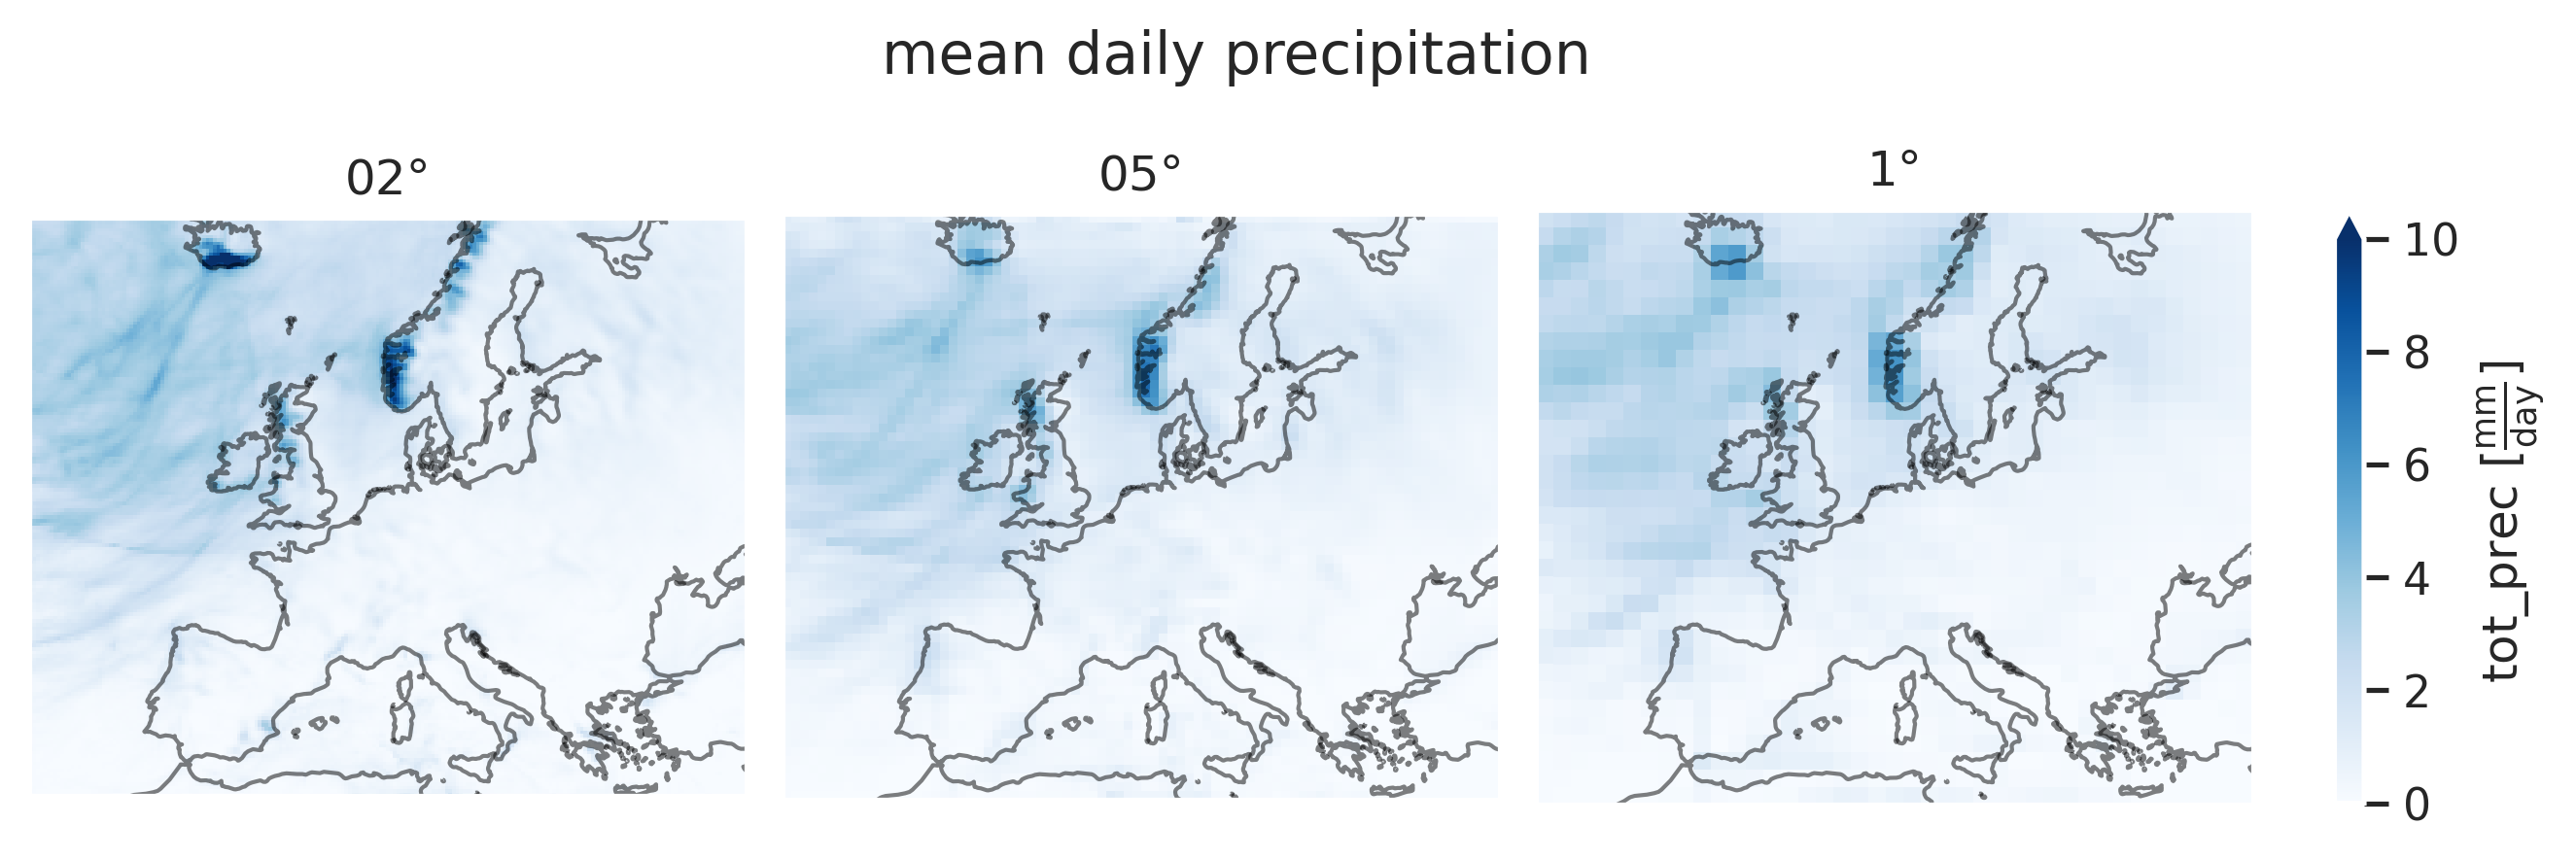
\includegraphics[width=\figwidth]{../figs/2-timmean.png}
	\caption{Temporal mean of daily precipitation sum for different grid resolutions. Simulations ran throughout January 1990.}
	\label{fig:timmean}
\end{figure}

\Cref{fig:timmean} illustrates the spatial distribution of mean precipitation: The general pattern of different grid resolutions is similar, depicting high precipitation rates over the Northern Atlantic and at the coasts of Iceland, Norway and Scotland. However, it is evident that high grid resolution locally increases the intensity of precipitation.

\begin{figure}
	\centering
	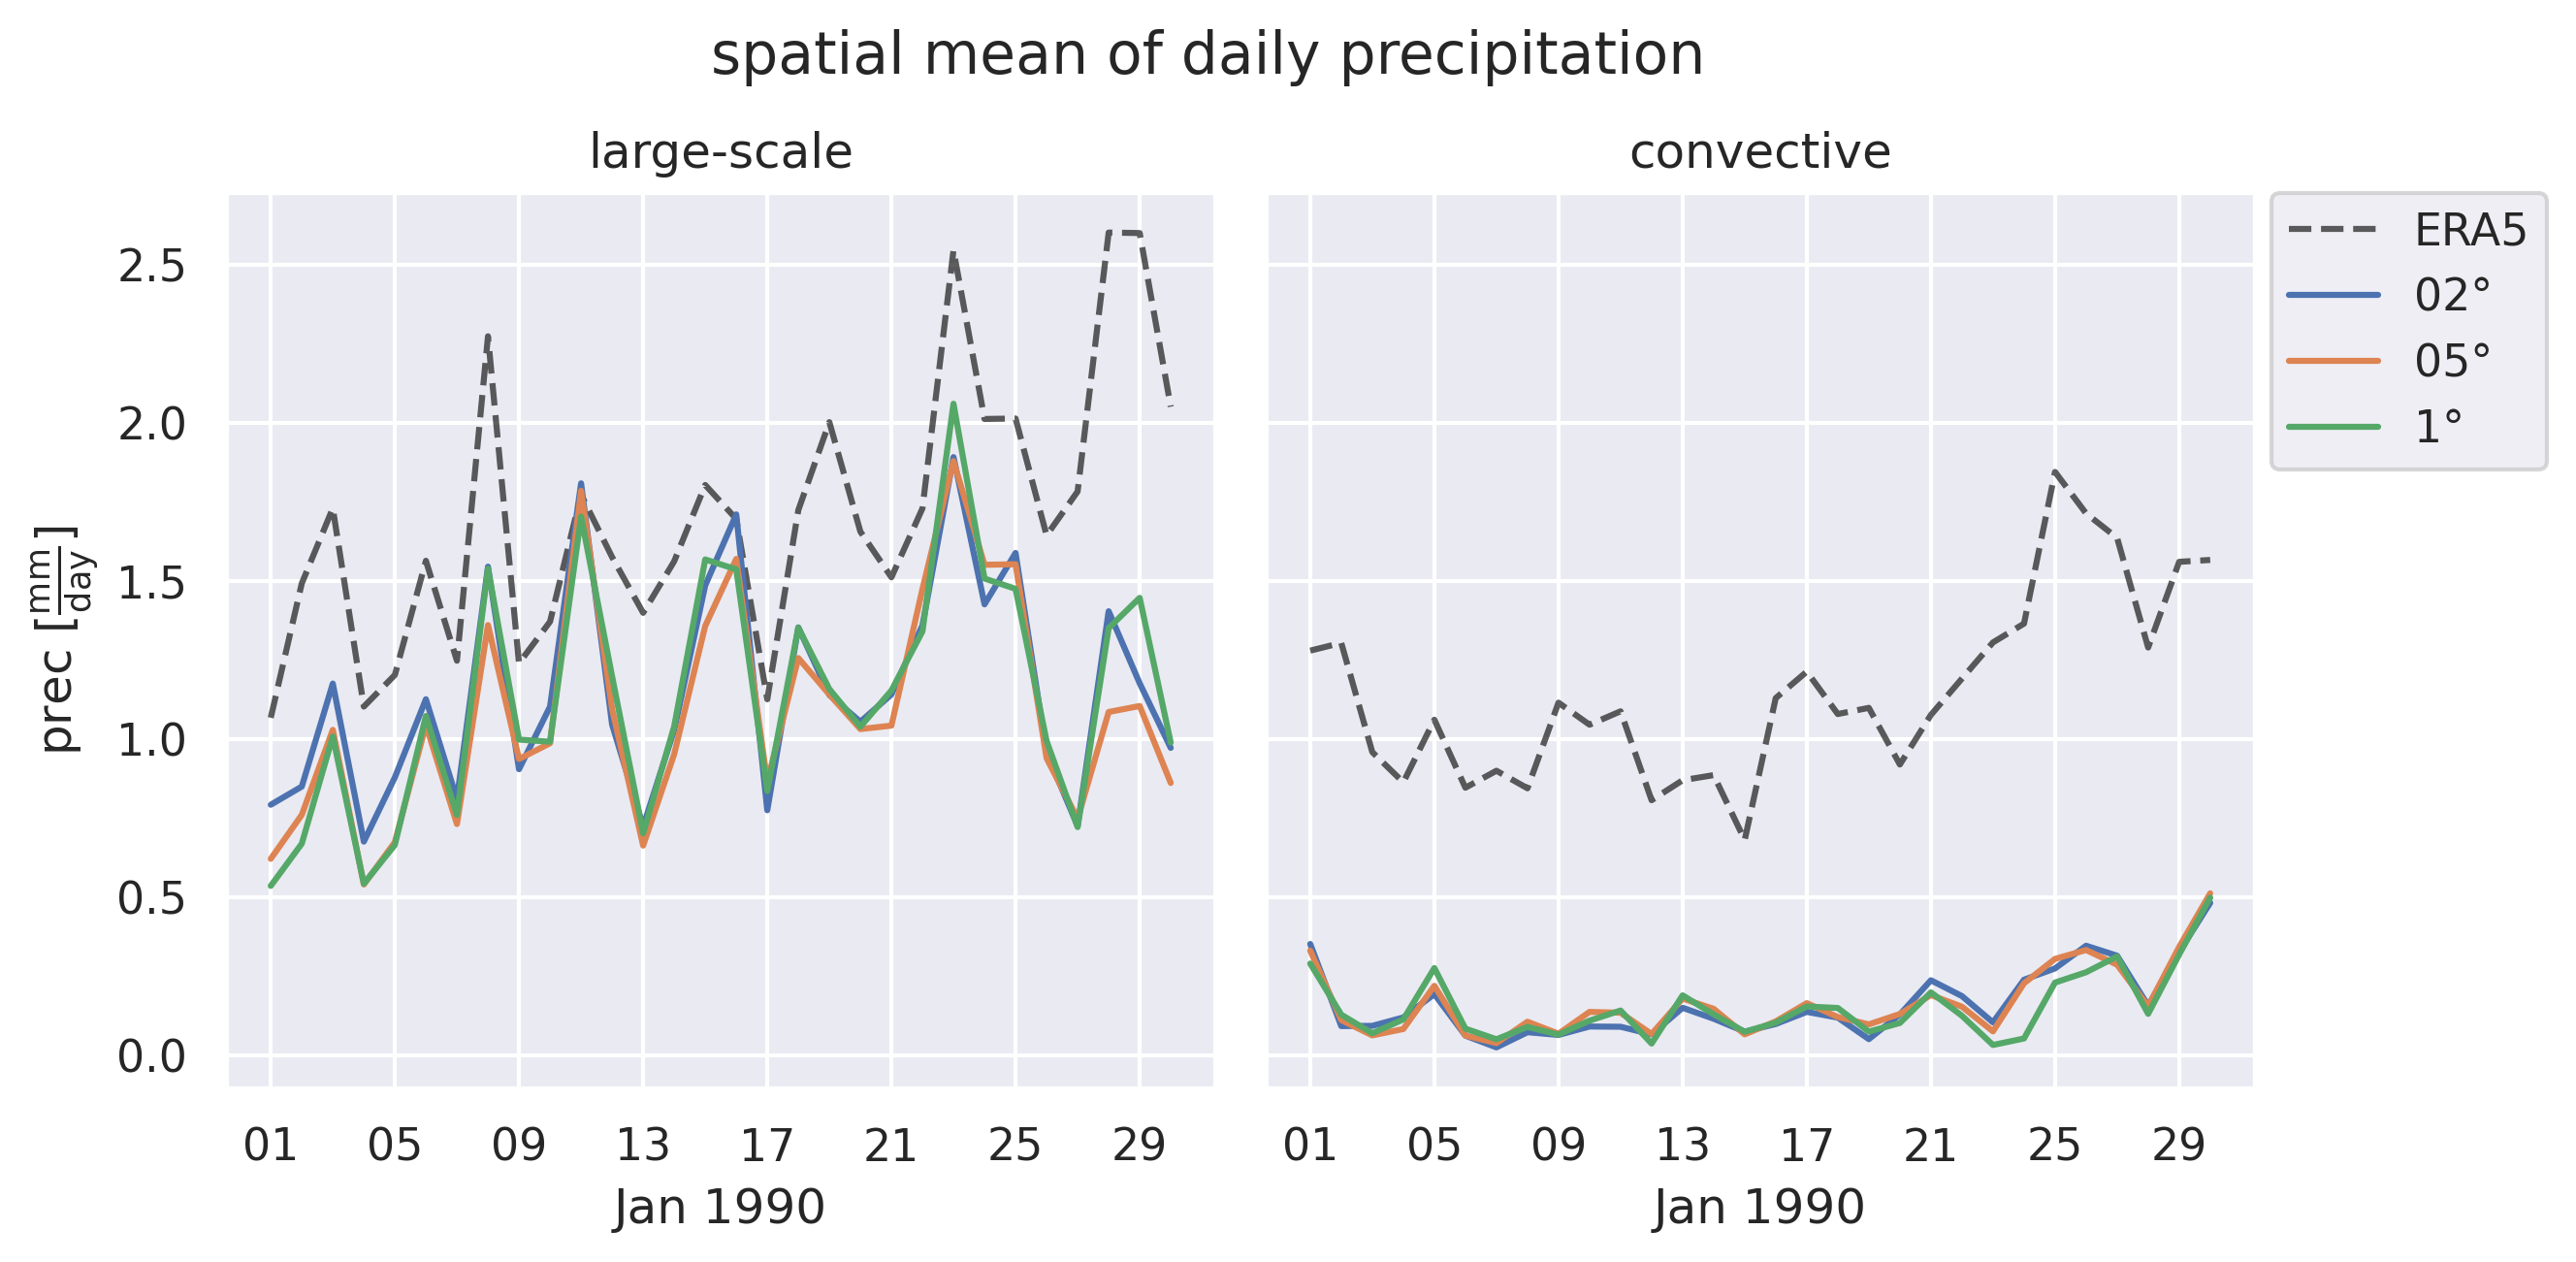
\includegraphics[width=\figwidth]{../figs/5-gsp-con.png}
	\caption{Spatial mean of daily precipitation sum split into large-scale (i.e., grid-scale) and convective signal for different grid resolutions. ERA5 reanalysis data as reference.}
	\label{fig:fldmean}
\end{figure}

When focussing on the temporal domain, the daily precipitation signals of the COSMO-CLM simulations are---generally speaking---similar, indicating that the daily sum over the entire (cropped) model region does not change considerably with model resolution. In \cref{fig:fldmean}, precipitation is split into a grid-scale and convective component, and ERA5 data is included as a reference.
In both subplots, simulations underestimate the observed daily precipitation sum, although the difference between reference and simulation is more pronounced for convective precipitation. The underlying trend in reference and simulation of grid-scale precipitation is comparable, which validates the model results on broader scales. It is important to note though that the simulations have been driven with ERA-Interim data and are now compared to ERA5 data, which might introduce additional biases triggered by different data assimilation procedures of the reanalyses.

The \textit{absolute} difference in precipitation between grid resolutions is more pronounced in the grid-scale precipitation, although without a consistent signal. E.g., in the beginning of January, 0.2°-resolution shows more grid-scale precipitation compared to the remaining resolutions, in the end of the month though, 0.2°- and 1°-resolution show a similar signal, while 0.5°-resolution simulates less grid-scale precipitation. In contrast, variation in the convective part is relatively small. I figure that the missing deep convection scheme is the reason, since all convective precipitation is derived from vertical turbulance only. Consequently